\documentclass[11pt,oneside]{article}	%use"amsart"insteadof"article"forAMSLaTeXformat
\usepackage{geometry}		%Seegeometry.pdftolearnthelayoutoptions.Therearelots.
\geometry{letterpaper}		%...ora4paperora5paperor...
%\geometry{landscape}		%Activateforforrotatedpagegeometry
%\usepackage[parfill]{parskip}		%Activatetobeginparagraphswithanemptylineratherthananindent
\usepackage{graphicx}				%Usepdf,png,jpg,orepsßwithpdflatex;useepsinDVImode
								%TeXwillautomaticallyconverteps-->pdfinpdflatex		
\usepackage{amssymb}
\usepackage{amsmath}
\usepackage{amsthm}
\newtheorem{definition}{Definition}
\newtheorem{theorem}{Theorem}

\usepackage[colorlinks]{hyperref}

%----macros begin-----------------------------------------------------------------------------------
\usepackage{graphicx}
\usepackage{color}
\usepackage{amsthm}

%\renewenvironment{Shaded}{\pause\begin{snugshade}}{\end{snugshade}}
\def\twocolumns#1#2{\begin{columns}
\begin{column}{0.5\linewidth}#1\end{column}
\begin{column}{0.5\linewidth}#2\end{column}
\end{columns}}
\def\mytwocolumns#1#2#3#4{\begin{columns}
\begin{column}{#1\linewidth}#2\end{column}
\begin{column}{#3\linewidth}#4\end{column}
\end{columns}}
\def\mythreecolumns#1#2#3#4#5#6{\begin{columns}
\begin{column}{#1\linewidth}#2\end{column}
\begin{column}{#3\linewidth}#4\end{column}
\begin{column}{#5\linewidth}#6\end{column}
\end{columns}}
\def\threecolumns#1#2#3{\begin{columns}
\begin{column}{0.33\linewidth}#1\end{column}
\begin{column}{0.33\linewidth}#2\end{column}
\begin{column}{0.33\linewidth}#3\end{column}
\end{columns}}
\def\fourcolumns#1#2#3#4{\begin{columns}%
\begin{column}{0.25\linewidth}#1\end{column}%
\begin{column}{0.25\linewidth}#2\end{column}%
\begin{column}{0.25\linewidth}#3\end{column}%
\begin{column}{0.25\linewidth}#4\end{column}%
\end{columns}}

\def\conv{\mbox{\textrm{conv}\,}}
\def\aff{\mbox{\textrm{aff}\,}}
\def\E{\mathbb{E}}
\def\R{\mathbb{R}}
\def\Z{\mathbb{Z}}
\def\tex{\TeX}
\def\latex{\LaTeX}
\def\v#1{{\bf #1}}
\def\p#1{{\bf #1}}
\def\T#1{{\bf #1}}

\def\vet#1{{\left(\begin{array}{cccccccccccccccccccc}#1\end{array}\right)}}
\def\mat#1{{\left(\begin{array}{cccccccccccccccccccc}#1\end{array}\right)}}

\def\lin{\mbox{\rm lin}\,}
\def\aff{\mbox{\rm aff}\,}
\def\pos{\mbox{\rm pos}\,}
\def\cone{\mbox{\rm cone}\,}
\def\conv{\mbox{\rm conv}\,}
\newcommand{\homog}[0]{\mbox{\rm homog}\,}
\newcommand{\relint}[0]{\mbox{\rm relint}\,}

%----macros end-----------------------------------------------------------------------------------

\usepackage{listings}

% Python style for highlighting
\lstset{
language=Python,
basicstyle=\ttm,
otherkeywords={self},             % Add keywords here
keywordstyle=\ttb\color{deepblue},
emph={MyClass,__init__},          % Custom highlighting
emphstyle=\ttb\color{deepred},    % Custom highlighting style
stringstyle=\color{deepgreen},
frame=tb,                         % Any extra options here
showstringspaces=false            % 
}


\title{The \texttt{smplxn} module
\footnote{This document is part of the framework~\cite{cclar-proj:2013:00}. \today}
}
\author{Alberto Paoluzzi}
%\date{}							%Activatetodisplayagivendateornodate

\begin{document}
\maketitle
\nonstopmode

\begin{abstract}
This module defines a minimal set of functions to generate a dimension-independent grid of simplices.
The name of the library was firstly used by our CAD Lab at University of Rome ``La Sapienza'' in years 1987/88 when we started working with dimension-independent simplicial complexes~\cite{Paoluzzi:1993:DMS:169728.169719}. This one in turn imports some functions from the \texttt{scipy} package and the geometric library \texttt{pyplasm}~\cite{}.
\end{abstract}

\tableofcontents\newpage

\section{Introduction}

The $Simple_X^n$ library, named \texttt{simplexn} within the Python version of the LARCC framework,
provides  combinatorial algorithms for some basic functions of geometric modelling with simplicial complexes. In particular, provides the efficient creation of simplicial complexes generated by simplicial complexes of lower dimension, the production of simplicial grids of any dimension, and the extraction of facets (i.e.~of $(d-1)$-faces) of complexes of $d$-simplices.

\section{Some simplicial algorithms}

The main aim of the simplicial functions given in this library is to provide optimal combinatorial algorithms, whose time complexity is linear in the size of the output.
Such a goal is achieved by calculating each cell in the output via closed combinatorial formulas, that do not require any searching nor data structure traversal to produce their results.

\subsection{Linear extrusion of a complex}

Here we discuss an implementation of the linear extrusion of simplicial complexes according to the method discussed in~\cite{Paoluzzi:1993:DMS:169728.169719} and~\cite{DBLP:journals/cad/FerruciP91}. In synthesis, for each $d$-simplex in the input complex, we generate combinatorially a $(d+1)$-simplicial \emph{tube}, i.e.~a chain of $d+1$ simplexes of dimension $d+1$. It can be shown that if the input simplices are a simplicial complex, then the output simplices are a complex too. 

In other words, if the input is a complex, where all $d$-cells either intersect along a common face or are pairwise disjoints, then the output is also a simplicial complex of dimension $d+1$. This method is computationally optimal, since it does not require any search or traversal of data structures. The algorithm~\cite{DBLP:journals/cad/FerruciP91} just writes the output making a constant number $O(1)$ of operation for each one of its $n$ output $d$-cells, so that the time complexity is $\Omega(n)$, where $n = d\,m$, being $m$ the number and $d$ the dimension (and the storage size) of the input cells, represented as lists of indices of vertices.

\paragraph{Computation}

Let us concentrate on the generation of the simplex chain $\gamma^{d+1}$ of dimension $d+1$ produced by combinatorial extrusion of a single simplex 
\[
\sigma^d = \langle v_0, v_1, \ldots, v_d,   \rangle .
\]
Then we have, with $|\gamma^{d+1}| = \sigma^d \times I$, and $I=[0,1]$:
\[
\gamma^{d+1} = \sum_{k=0}^{d} (-1)^{kd} \langle v_k, \ldots v_d, v^*_0, \ldots  v^*_k \rangle 
\]
with $v_k\in \sigma^d \times \{0\}$ and  $v^*_k\in \sigma^d \times \{1\}$, and where the term $(-1)^{kd}$ is used to generate a chain of coherently-oriented extruded simplices.

\begin{figure}[htbp] %  figure placement: here, top, bottom, or page
   \centering
   \begin{minipage}[c]{0.49\linewidth}
		\caption{Extrusion of (a) a point; (b) a straight line segment; (c) a triangle.}
	\end{minipage} 
   \begin{minipage}[c]{0.49\linewidth}
		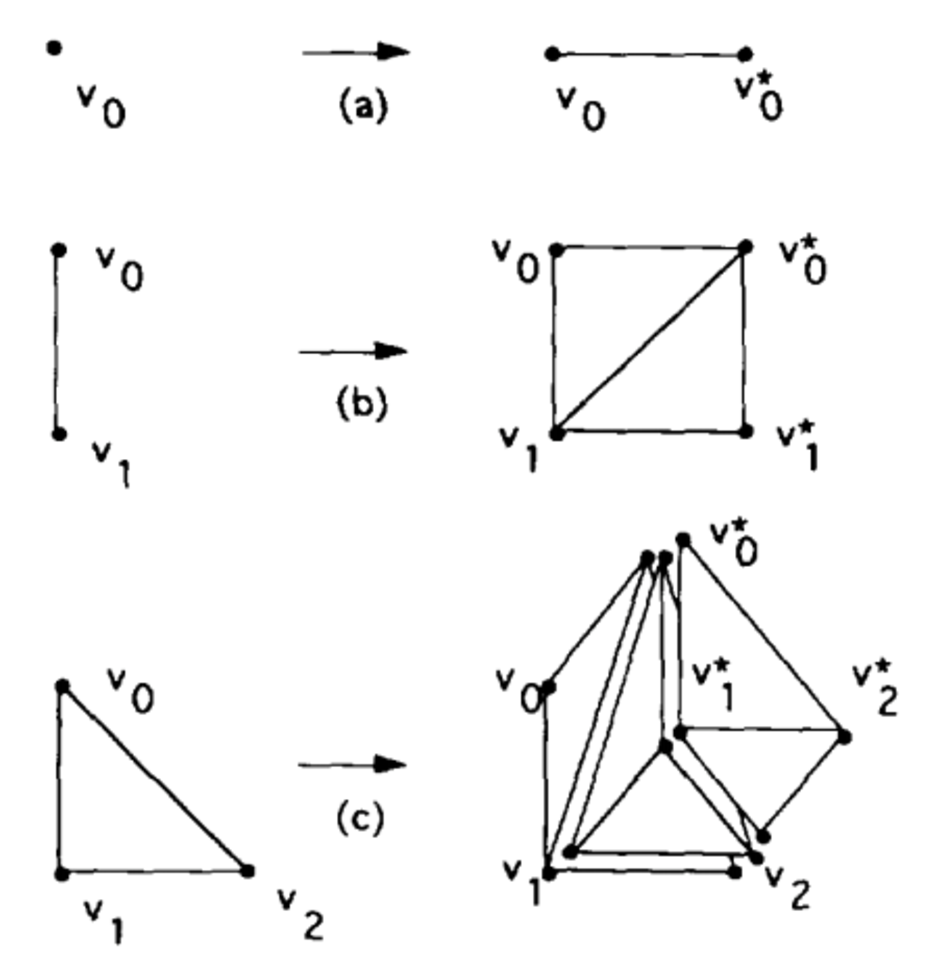
\includegraphics[width=0.8\linewidth]{images/extrusion}
	\end{minipage} 
   \label{fig:extrusion}
\end{figure}

In our implementation the combinatorial algorithm above is twofold generalised:
\begin{enumerate}
\item by applying it to all $d$-simplices of a LAR model of dimension $d$;
\item by using instead of the single interval $I=[0,1]$, the possibly unconnected set of 1D intervals generated by the list of integer numbers stored in the \texttt{pattern} variable
\end{enumerate}

\paragraph{Implementation}
In the macro below, \texttt{larExtrude} is the function to generate the output model vertices in a multiple extrusion of a LAR model.

First we notice that the \texttt{model} variable contains a pair (\texttt{V}, \texttt{FV}), where \texttt{V} is the array of input vertices, and \texttt{FV} is the array of $d$-cells (given as lists of vertex indices) providing the  input representation of a LAR cellular complex.

The \texttt{pattern} variable is a list of integers, whose absolute values provide the sizes of the ordered set of 1D (in local coords) subintervals specified by the \texttt{pattern} itself. Such subintervals are assembled in global coordinates, and each one of them is considered either solid or void depending on the sign of the corresponding integer, which may be either positive (solid subinterval) or negative (void subinterval).  

Therefore, a value \texttt{pattern = [1,1,-1,1]} must be interpreted as the 1D simplicial complex
\[
[0,1] \cup [1,2] \cup [3,4]
\]
with five vertices \texttt{W = [[0.0], [1.0], [2.0], [3.0], [4.0]]} and three $1$-cells \texttt{[[0,1], [1,2], [3,4]]}.

\texttt{V} is the list of input $d$-vertices (each given as a list of $d$ coordinates);
\texttt{coords} is a list of absolute translation parameters to be applied to \texttt{V} in order to generate the output vertices generated by the combinatorial extrusion algorithm.

The \texttt{cellGroups} variable is used to select the groups of $(d+1)$-simplices corresponding to solid intervals in the input \texttt{pattern}, and \texttt{CAT} provides to flatten their set, by removing a level of square brackets.

%-------------------------------------------------------------------------------
@d Simplicial model extrusion in accord with a 1D pattern
@{def larExtrude(model,pattern):
    V, FV = model
    d, m = len(FV[0]), len(pattern)
    coords = list(cumsum([0]+(AA(ABS)(pattern))))
    offset, outcells, rangelimit = len(V), [], d*m
    for cell in FV:
        @< Append a chain of extruded cells to outcells @>
    outcells = AA(CAT)(TRANS(outcells))
    cellGroups = [group for k,group in enumerate(outcells) if pattern[k]>0 ]
    outVertices = [v+[z] for z in coords for v in V]
    outModel = outVertices, CAT(cellGroups)
    return outModel
@}
%-------------------------------------------------------------------------------

\paragraph{Extrusion of single cells}
For each cell in \texttt{FV} a chain of vertices is created, then they are separated into groups of $d+1$ consecutive elements, by shifting one position at a time.

%-------------------------------------------------------------------------------
@d Append a chain of extruded cells to outcells
@{@< Create the indices of vertices in the cell "tube" @>
@< Take groups of d+1 elements, by shifting one position @>	
@}
%-------------------------------------------------------------------------------

\paragraph{Assembling vertex indices in a tube with their shifted images}
Here the ``long'' chain of vertices is created.
%-------------------------------------------------------------------------------
@d Create the indices of vertices in the cell "tube"
@{tube = [v + k*offset for k in range(m+1) for v in cell]	@}
%-------------------------------------------------------------------------------

\paragraph{Selecting and reshaping extruded cells in a tube}
Here the chain of vertices is spitted into subchains, and such subchains are reshaped into three-dimensional arrays of indices.
%-------------------------------------------------------------------------------
@d Take groups of d+1 elements, by shifting one position
@{cellTube = [tube[k:k+d+1] for k in range(rangelimit)]
outcells += [reshape(cellTube, newshape=(m,d,d+1)).tolist()]	@}
%-------------------------------------------------------------------------------



\begin{definition}[Big-Omega order]
We say that a function $f(n)$ is \emph{Big-Omega} order of a function $f(n)$, and write 
$f(n) \in \Omega(g(n))$ when a constant $c$ exists, such that:
\[
\lim_{n\to\infty} \frac{f(n)}{g(n)}=c>0,\qquad \mbox{where\ } 0<c\leq\infty.
\]
\end{definition}



\begin{theorem}[Optimality]
The combinatorial algorithm for extrusion of simplicial complexes has time complexity $\Omega(n)$.
\end{theorem}
\proof{
Of course, if we denote as $g(n) = nd$ the time needed to write the input of the extrusion algorithm, proportional to the constant length $d$ of cells, and as $f(m) = m(d+1)$ the time needed to write the output, where $m=n(d+1)$, we have
\[
\lim_{n\to\infty} \frac{f(n)}{g(n)}= \lim_{n\to\infty} \frac{m(d+1)}{nd}
= \lim_{n\to\infty} \frac{[n(d+1)](d+1)}{nd} = \frac{(d+1)^2}{d} = c > 0
\]
\qed}

\subsubsection{Examples of simplicial complex extrusions}

\paragraph{Example 1}
It is interesting to notice that the 2D model extruded in example 1 below and shown in Figure~\ref{fig:assembly} is locally non-manifold, and that several instance of the pattern in the $z$ direction are obtained by just inserting a void subinterval (negative size) in the \texttt{pattern} value.

\begin{figure}[htbp] %  figure placement: here, top, bottom, or page
   \centering
   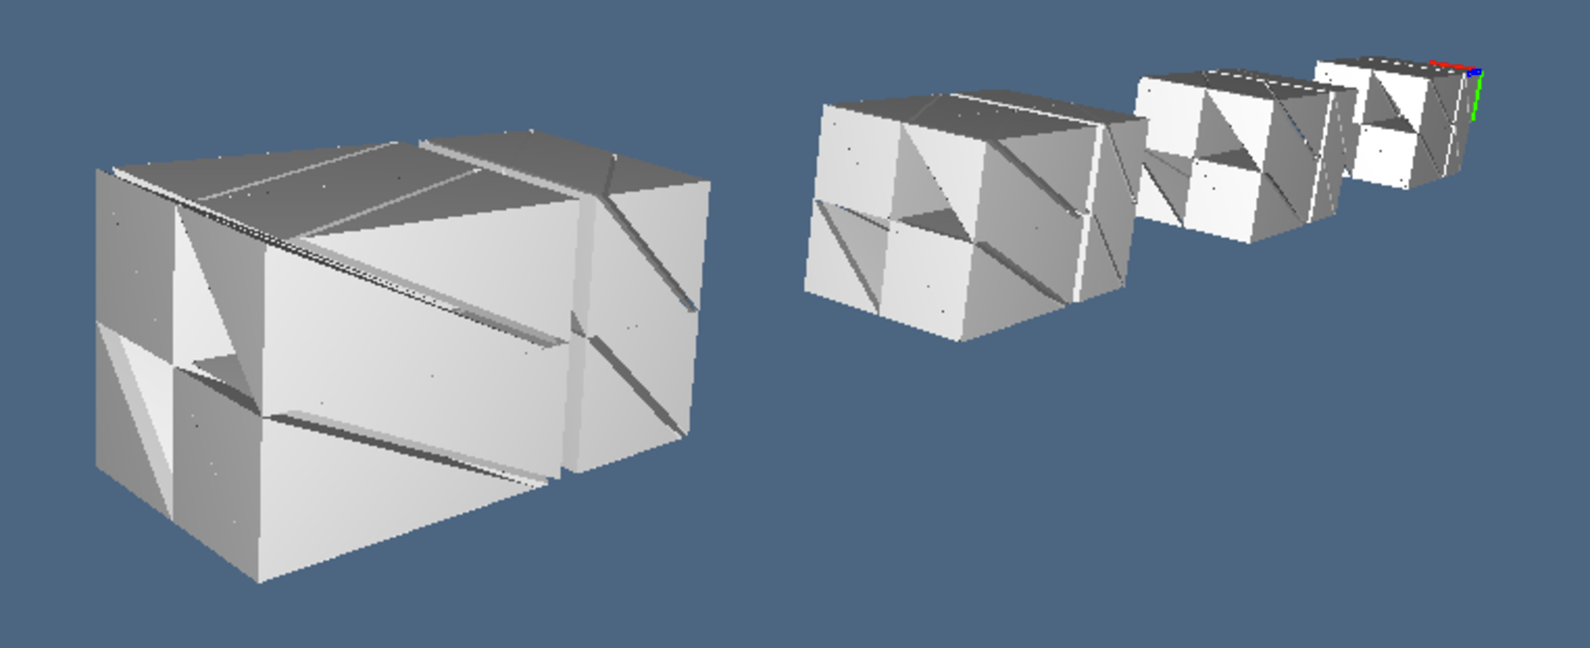
\includegraphics[width=0.7\linewidth]{images/assembly} 
   \caption{A simplicial complex providing a quite complex 3D assembly of tetrahedra.}
   \label{fig:assembly}
\end{figure}

\paragraph{Examples 2 and 3}
The examples show that the implemented \texttt{larExtrude} algorithm is fully multidimensional. 
It may be worth noting the initial definition of the empty \texttt{model}, as a pair having the empty list as vertex set and the list \texttt{[[0]]} as the cell list. Such initial value is used
to define a predefinite constant \texttt{VOID}.

\begin{figure}[htbp] %  figure placement: here, top, bottom, or page
   \centering
   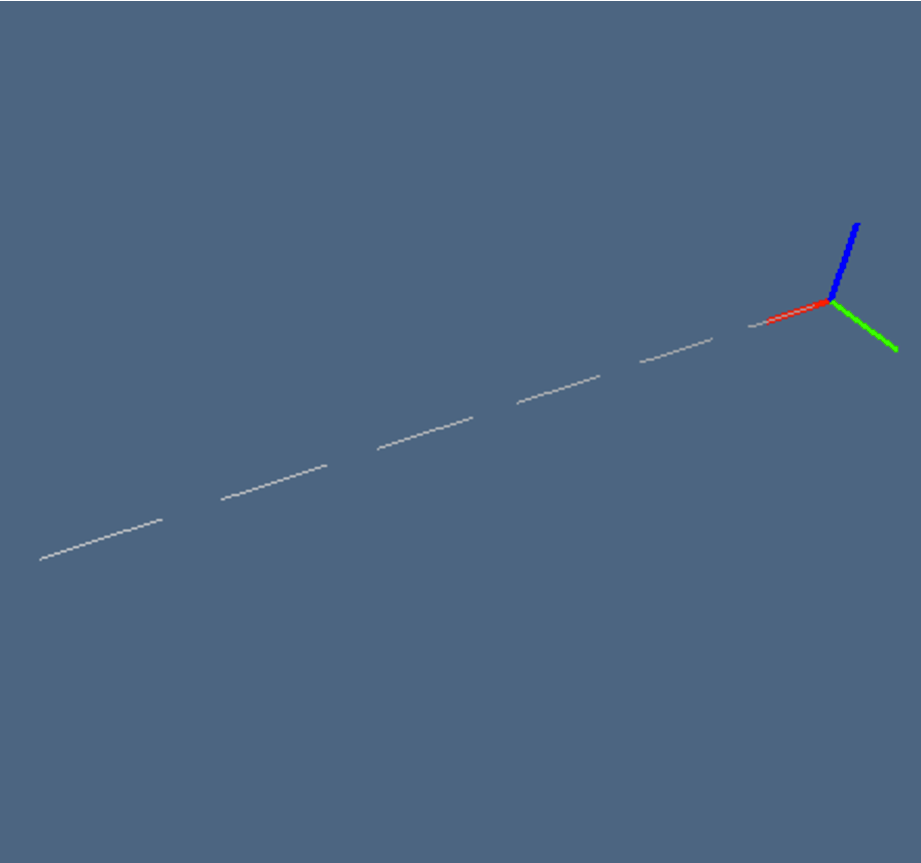
\includegraphics[height=0.25\linewidth,width=0.25\linewidth]{images/simplexn-1a} 
   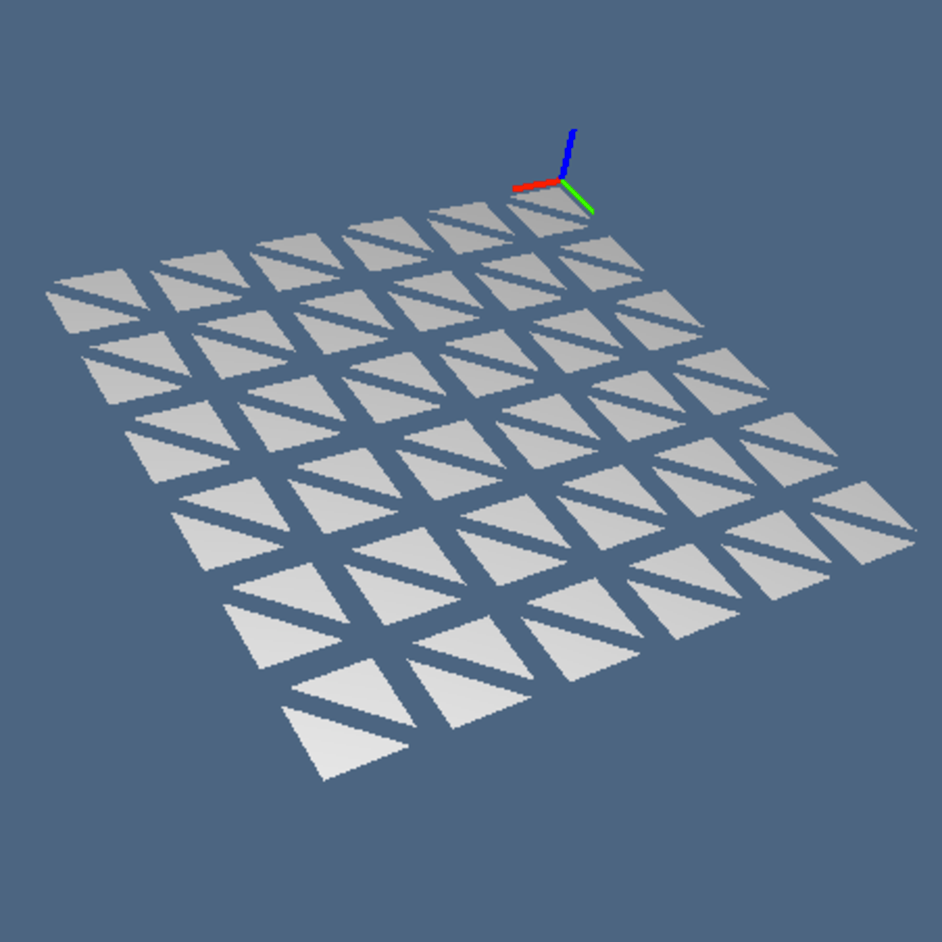
\includegraphics[height=0.25\linewidth,width=0.25\linewidth]{images/simplexn-1b} 
   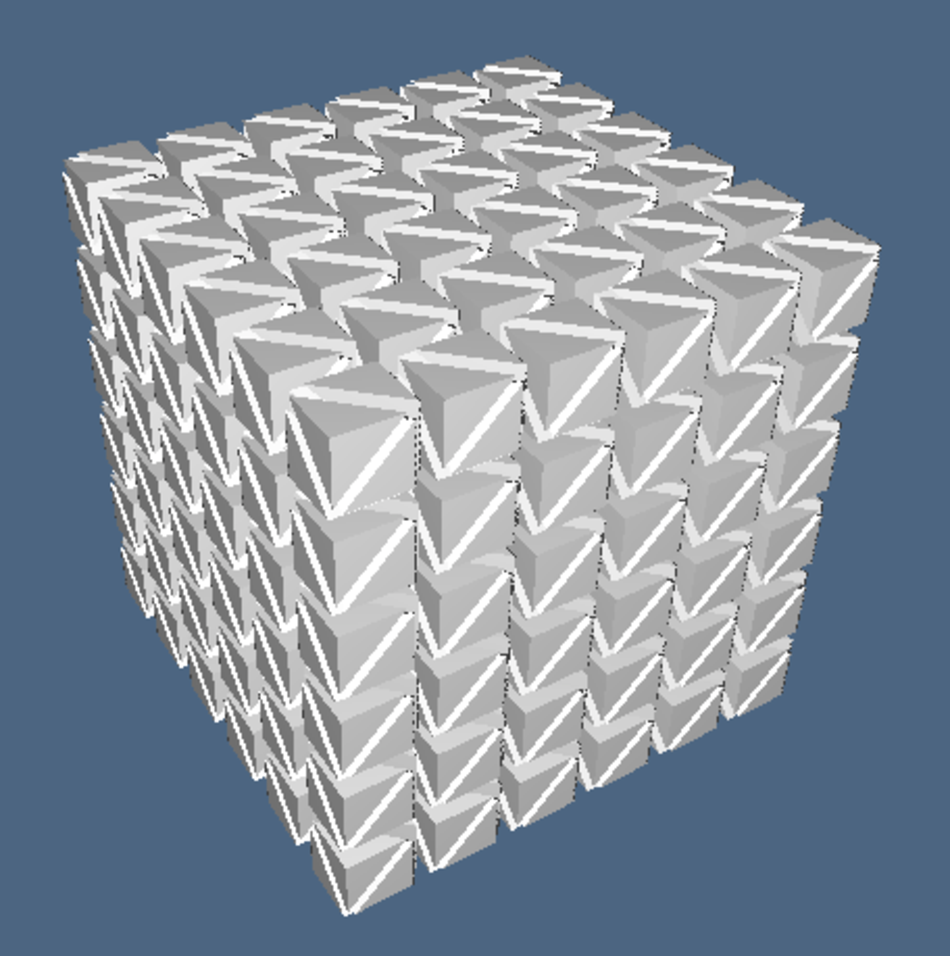
\includegraphics[height=0.25\linewidth,width=0.25\linewidth]{images/simplexn-1c} 
   \caption{1-, 2-, and 3-dimensional simplicial complex generated by repeated extrusion with the same pattern.}
   \label{fig:example}
\end{figure}

%-------------------------------------------------------------------------------
@D Examples of simplicial complex extrusions
@{# example 1
V = [[0,0],[1,0],[2,0],[0,1],[1,1],[2,1],[0,2],[1,2],[2,2]]
FV = [[0,1,3],[1,2,4],[2,4,5],[3,4,6],[4,6,7],[5,7,8]]
model = larExtrude((V,FV),4*[1,2,-3])
VIEW(EXPLODE(1,1,1.2)(MKPOLS(model)))

# example 2
model = larExtrude( VOID, 6*[1] )
VIEW(EXPLODE(1.5,1.5,1.5)(MKPOLS(model)))
model = larExtrude( model, 6*[1] )
VIEW(EXPLODE(1.5,1.5,1.5)(MKPOLS(model)))
model = larExtrude( model, 6*[1] )
VIEW(EXPLODE(1.5,1.5,1.5)(MKPOLS(model)))

# example 3
model = larExtrude( VOID, 10*[1,-1] )
VIEW(EXPLODE(1.5,1.5,1.5)(MKPOLS(model)))
model = larExtrude( model, 10*[1] )
VIEW(EXPLODE(1.5,1.5,1.5)(MKPOLS(model)))
@}
%-------------------------------------------------------------------------------


\begin{figure}[htbp] %  figure placement: here, top, bottom, or page
   \centering
   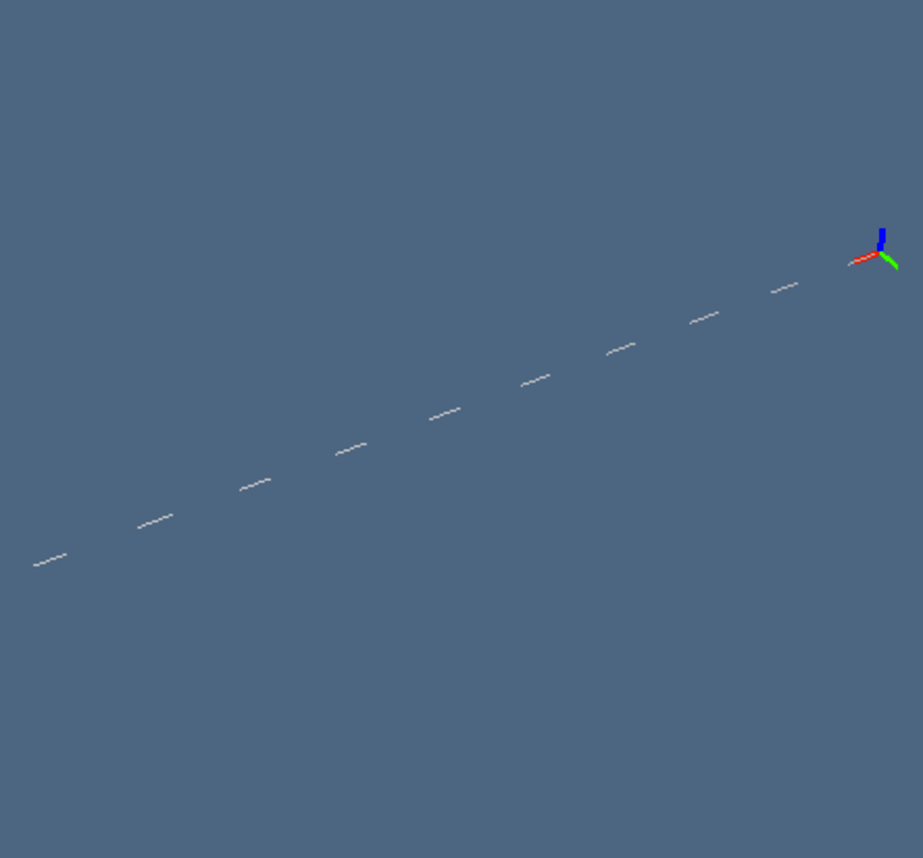
\includegraphics[height=0.25\linewidth,width=0.25\linewidth]{images/simplexn-2a} 
   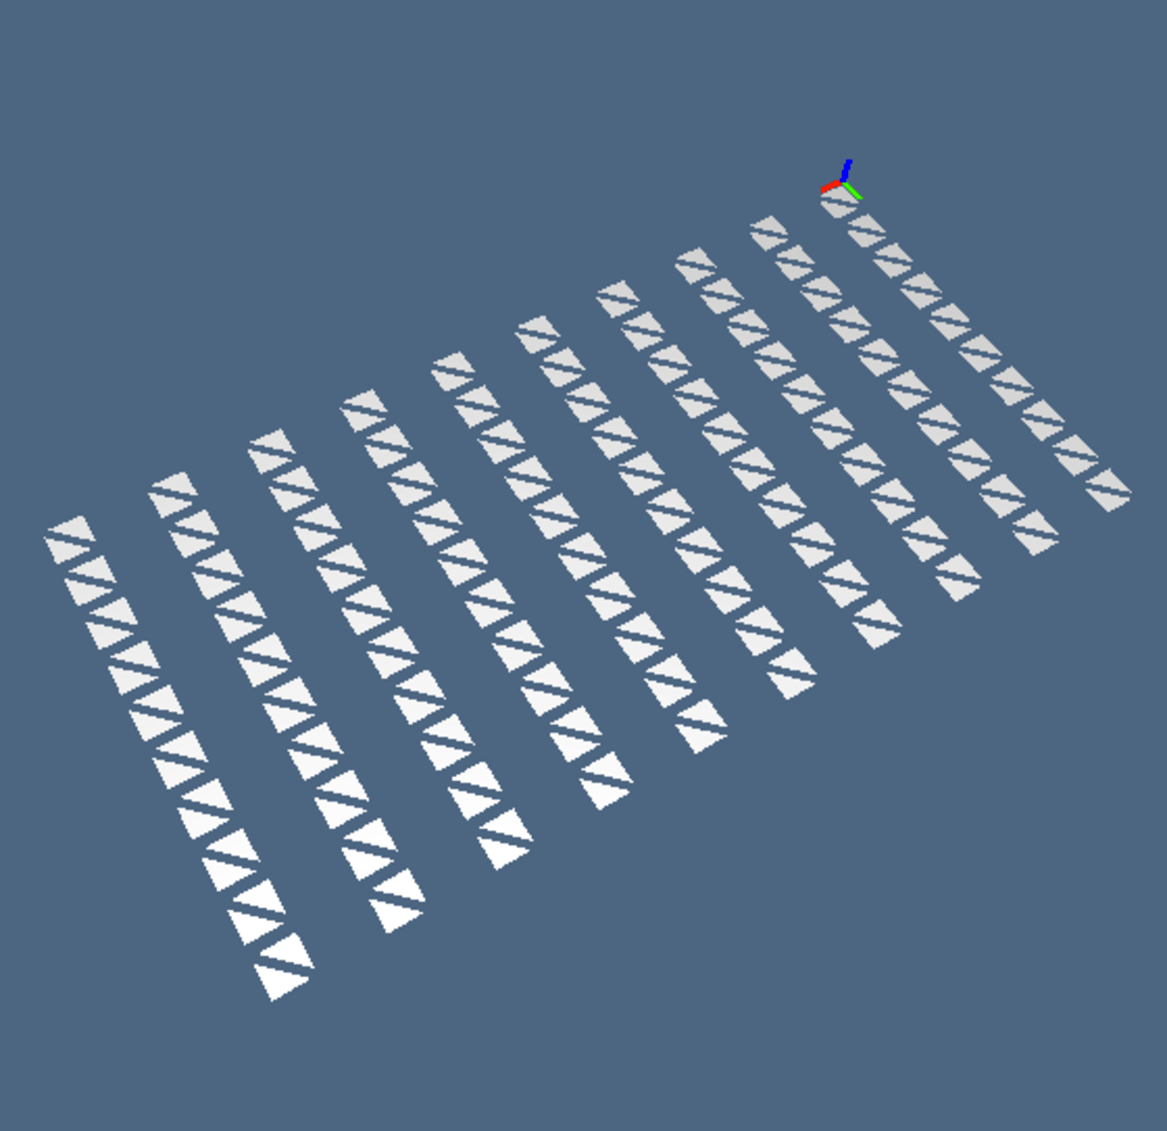
\includegraphics[height=0.25\linewidth,width=0.25\linewidth]{images/simplexn-2b} 
   \caption{1- and 2-dimensional simplicial complexes generated by different patterns.}
   \label{fig:example}
\end{figure}


\subsection{Generation of multidimensional simplicial grids}

The generation of simplicial grids of any dimension and shape using the \texttt{larSimplexGrid}
is amazingly simple. The input parameter \texttt{shape} is either a tuple or a list of integers used to specify the \emph{shape} of the created array, i.e.~both the number of its dimensions (given by \texttt{len(shape)}) and the \texttt{size} of each dimension $k$ (given by the \texttt{shape[k]} element).
The implementation starts from the LAR model of the void simplicial complex (denoted as \texttt{VOID}, a predefined constant) and updates the \texttt{model} variable extruding it iteratively according to the specs given by \texttt{shape}.
Just notice that the returned grid \texttt{model} has vertices with integer coordinates, that can be subsequently scaled and/or translated and/or mapped in any other way, according to the user needs.

%-------------------------------------------------------------------------------
@d Generation of simplicial grids
@{def larSimplexGrid(shape):
    model = VOID
    for item in shape:
        model = larExtrude(model,item*[1])
    return model
@}
%-------------------------------------------------------------------------------


\paragraph{Examples of simplicial grids} The two examples of simplicial grids generated by the macro below with \texttt{shape} equal to \texttt{[3,3]} and \texttt{[2,3,4]}, respectively, are displayed in Figure~\ref{fig:simplexn-3}.

\begin{figure}[htbp] %  figure placement: here, top, bottom, or page
   \centering
   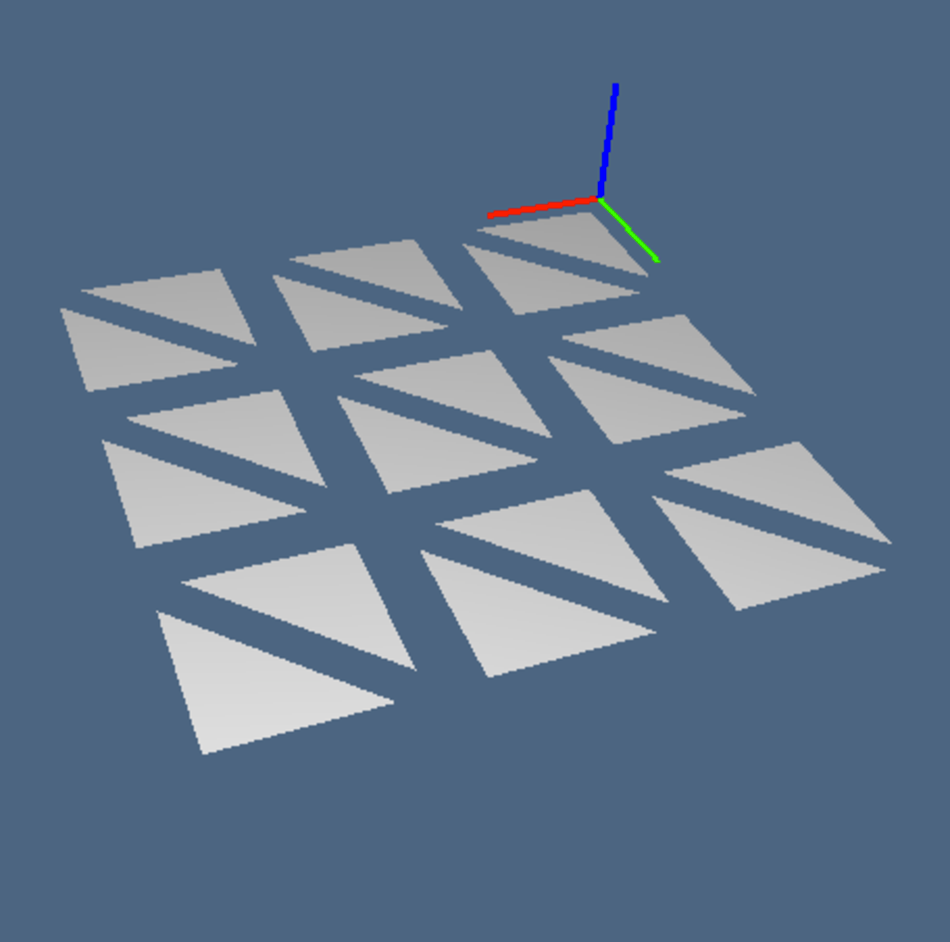
\includegraphics[height=0.25\linewidth,width=0.25\linewidth]{images/simplexn-3a} 
   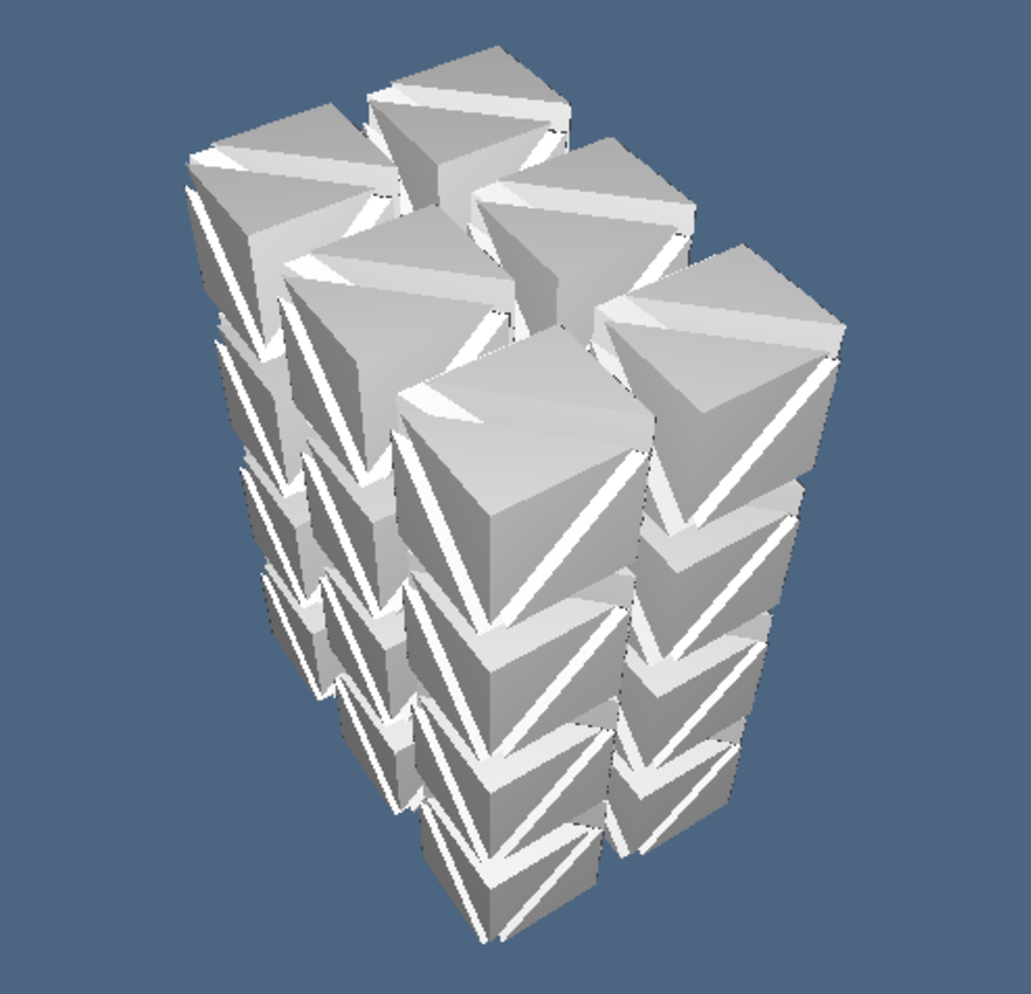
\includegraphics[height=0.25\linewidth,width=0.25\linewidth]{images/simplexn-3b} 
   \caption{2- and 3-dimensional simplicial grids.}
   \label{fig:simplexn-3}
\end{figure}

%-------------------------------------------------------------------------------
@d Examples of simplicial grids
@{grid_2d = larSimplexGrid([3,3])
VIEW(EXPLODE(1.5,1.5,1.5)(MKPOLS(grid_2d)))

grid_3d = larSimplexGrid([2,3,4])
VIEW(EXPLODE(1.5,1.5,1.5)(MKPOLS(grid_3d)))
@}
%-------------------------------------------------------------------------------


\subsection{Facet extraction from simplices}

A $k$-face of a $d$-simplex is defined as the convex hull of any subset of $k$ vertices.
A $(d-1)$-face of a $d$-simplex 
\[
\sigma^d = \langle v_0, v_1, \ldots, v_d \rangle
\]
 is also called a \emph{facet}. Each of the $d+1$ facets of $\sigma^d$, obtained by removing a vertex from $\sigma^d$, is a $(d-1)$-simplex. A simplex may be oriented in two different ways according to the permutation
class of its vertices. The simplex \emph{orientation} is so changed by either multiplying the simplex by -1, or by executing an odd number of exchanges of its vertices. 

The chain of oriented boundary facets of $\sigma^d$, usually denoted as $\partial \sigma^d$, is generated combinatorially as follows:
\[
\partial\, \sigma^d = \sum_{k=0}^d (-1)^d \langle v_0, \ldots, v_{k-1}, v_{k+1}, \ldots, v_d \rangle
\]

\paragraph{Implementation}

The \texttt{larSimplexFacets} function, for estraction of non-oriented $(d-1)$-facets of $d$-dimensional simplices, returns a list of $d$-tuples of integers, i.e.~the input LAR representation of the topology of a cellular complex. The final \emph{list comprehension} is used to remove the duplicated facets, by taking only the last element of any subsequence with possibly duplicated elements.
        
%-------------------------------------------------------------------------------
@d Facets extraction from a set of simplices
@{def larSimplexFacets(simplices):
    out = []
    d = len(simplices[0])
    for simplex in simplices:
        out += [simplex[0:k]+simplex[k+1:d] for k in range(d)]
    out = sorted(out)
    return [facet for k,facet in enumerate(out[:-1]) if out[k] != out[k+1]] \
    	+ [out[-1]] 
@}
%-------------------------------------------------------------------------------

\paragraph{Examples of facet extraction}
The simple generation of the LAR model of a simplicial decomposition of a 3D cube as a \texttt{larSimplexGrid} with \texttt{shape = [1,1,1]} and of its 2D and 1D skeletons is shown here.

%-------------------------------------------------------------------------------
@d Examples of facet extraction from 3D simplicial cube
@{V,CV = larSimplexGrid([1,1,1])
VIEW(EXPLODE(1.5,1.5,1.5)(MKPOLS((V,CV))))
SK2 = (V,larSimplexFacets(CV))
VIEW(EXPLODE(1.5,1.5,1.5)(MKPOLS(SK2)))
SK1 = (V,larSimplexFacets(SK2[1]))
VIEW(EXPLODE(1.5,1.5,1.5)(MKPOLS(SK1)))
@}
%-------------------------------------------------------------------------------



\subsection{Exporting the $Simple_x^n$ library}
The current version of the \texttt{simplexn} library is exported here. Next versions will take care of the OpenCL acceleration and data partitioning with very-large size simplicial grids and their sets of faces.

%-------------------------------------------------------------------------------
@o lib/py/simplexn.py 
@{# -*- coding: utf-8 -*-
"""Module for facet extraction, extrusion and simplicial grids"""
from lar2psm import *
from scipy import *

VOID = V0,CV0 = [[]],[[0]]    # the empty simplicial model
@< Cumulative sum  @>
@< Simplicial model extrusion in accord with a 1D pattern @>
@< Generation of simplicial grids @>
@< Facets extraction from a set of simplices @>
if __name__ == "__main__":
	@< Examples of simplicial complex extrusions @>
	@< Examples of simplicial grids @>
	@< Examples of facet extraction from 3D simplicial cube @>
@}
%-------------------------------------------------------------------------------


\section{Signed (co)boundary matrices of a simplicial complex}
\label{simplicial}

\section{Test examples}

\subsection{Structured grid}

\subsubsection{2D example}

\paragraph{Generate a simplicial decomposition}
Then we generate and show a 2D decomposition of the unit square $[0,1]^2\subset\E^2$ into a $3\times 3$ grid of simplices (triangles, in this case), using the \texttt{larSimplexGrid} function, that returns a pair \texttt{(V,FV)}, made by the array \texttt{V} of vertices, and by the array \texttt{FV} of ``faces by vertex'' indices, that constitute a \emph{reduced} simplicial LAR of the $[0,1]^2$ domain. The computed \texttt{FV} array is then dispayed ``exploded'', being $ex,ey,ez$ the explosion parameters in the $x,y,z$ coordinate directions, respectively. Notice that the \texttt{MKPOLS} pyplasm primitive requires a pair \texttt{(V,FV)}, that we call a ``model'', as input --- i.e. a pair made by the array \texttt{V} of vertices, and by a zero-based array of array of indices of vertices. Elsewhere in this document we identified such a data structure as CSR$(M_d)$, for some dimension $d$. Suc notation stands for the Compressed Sparse Row representation of a binary characteristic matrix.

@d Generate a simplicial decomposition ot the $[0,1]^2$ domain
@{V,FV = larSimplexGrid([3,3])
VIEW(EXPLODE(1.5,1.5,1.5)(MKPOLS((V,FV))))
@}

\paragraph{Extract the $(d-1)$-faces}
Since the complex is simplicial, we can directly extract its facets (in this case the 1-faces, i.e. its edges) by invoking the \texttt{larSimplexFacets} function on the argument \texttt{FV}, so returning the array \texttt{EV} of ``edges by vertex'' indices. 

%-------------------------------------------------------------------------------
@d Extract the edges of the 2D decomposition
@{EV = larSimplexFacets(FV)
ex,ey,ez = 1.5,1.5,1.5
VIEW(EXPLODE(ex,ey,ez)(MKPOLS((V,EV))))
@}
%-------------------------------------------------------------------------------

\paragraph{Export the executable file}
We are finally able to generate and output a complete test file, including the visualization expressions. This file can be executed by the \texttt{test} target of the \texttt{make} command.

%-------------------------------------------------------------------------------
@O test/py/test01.py
@{
@<Inport the $Simple_X^n$ library@>
@<Generate a simplicial decomposition ot the $[0,1]^2$ domain@>
@<Extract the edges of the 2D decomposition@>
@}
%-------------------------------------------------------------------------------

\subsubsection{3D example}

In this case we produce a $2\times 2\times 2$ grid of tetrahedra. The dimension (3D) of the model to be generated is inferred by the presence of 3 parameters in the parameter list of the \texttt{larSimplexGrid} function. 

%-------------------------------------------------------------------------------
@d Generate a simplicial decomposition ot the $[0,1]^3$ domain
@{V,CV = larSimplexGrid([2,2,2])
VIEW(EXPLODE(1.5,1.5,1.5)(MKPOLS((V,CV))))
@}
%-------------------------------------------------------------------------------

and repeat two times the facet extraction:

%-------------------------------------------------------------------------------
@d Extract the faces and edges of the 3D decomposition
@{
FV = larSimplexFacets(CV)
VIEW(EXPLODE(1.5,1.5,1.5)(MKPOLS((V,FV))))
EV = larSimplexFacets(FV)
VIEW(EXPLODE(1.5,1.5,1.5)(MKPOLS((V,EV))))
@}
%-------------------------------------------------------------------------------

and finally export a new test file:

%-------------------------------------------------------------------------------
@O test/py/test02.py 
@{
@<Inport the $Simple_X^n$ library@>
@<Generate a simplicial decomposition ot the $[0,1]^3$ domain@>
@<Extract the faces and edges of the 3D decomposition@>
@}
%-------------------------------------------------------------------------------


\subsection{Unstructured grid}


\subsubsection{2D example}


\subsubsection{3D example}


\appendix
\section{Utilities}


%-------------------------------------------------------------------------------
@d Cumulative sum
@{
def cumsum(iterable):
    # cumulative addition: list(cumsum(range(4))) => [0, 1, 3, 6]
    iterable = iter(iterable)
    s = iterable.next()
    yield s
    for c in iterable:
        s = s + c
        yield s
@}
%-------------------------------------------------------------------------------


\bibliographystyle{amsalpha}
\bibliography{smplxn}

\end{document}
